\chapter{Sp\'ecification des besoins}
\label{chap:besoins}

\section{Introduction}

Ce chapitre traduit le p\'erim\`etre du prototype en besoins v\'erifiables. Les
exigences sont tir\'ees des contrats d'API, des contr\^oles d'entr\'ee, des vues
op\'erateur et des limites d\'eclar\'ees dans le d\'ep\^ot. Elles ne supposent ni
d\'eploiement de production ni compatibilit\'e NFStream en direct.

\section{Acteurs}

\begin{description}
  \item[Security Analyst / Administrator.] Op\'erateur humain qui s'authentifie,
  supervise le syst\`eme, contr\^ole le rejeu, examine les alertes, consulte les
  preuves des mod\`eles et enregistre une qualification.

  \item[External IoT system / sensor agent.] Syst\`eme externe qui transmet soit
  des observations de flux conformes au sch\'ema canonique, soit des \'ev\'enements
  Suricata avec le jeton r\'eserv\'e au capteur. L'attaquant n'est pas un acteur du
  logiciel: son activit\'e \'eventuelle est une donn\'ee observ\'ee par le syst\`eme.
\end{description}

\noindent\begin{minipage}{\textwidth}
\section{Besoins fonctionnels}

\begin{center}
  \captionsetup{type=table}
  \captionof{table}{Besoins fonctionnels du prototype}
  \label{tab:functional-requirements}
  \renewcommand{\arraystretch}{1.22}
  \rowcolors{2}{EmeraldWash}{white}
  \begin{tabularx}{\textwidth}{@{}>{\bfseries\color{PremiumEmerald}}p{0.12\textwidth}Y@{}}
    \ReportTableHeader{ID}{Besoin}
    BF-01 & Authentifier l'op\'erateur et prot\'eger les fonctions m\'etier par un jeton à dur\'ee limit\'ee. \\
    BF-02 & Valider puis accepter des observations de flux versionn\'ees en mode synchrone ou par ingestion durable. \\
    BF-03 & Ex\'ecuter la cascade binaire puis, uniquement pour une attaque, la classification de famille. \\
    BF-04 & Rejouer un sous-ensemble born\'e du jeu de donn\'ees et permettre la pause, la reprise et l'arr\^et. \\
    BF-05 & Persister les observations, pr\'edictions, alertes et transitions utiles à l'audit. \\
    BF-06 & Pr\'esenter, filtrer et d\'etailler les alertes puis enregistrer la qualification de l'analyste. \\
    BF-07 & Publier les nouvelles pr\'edictions et alertes aux tableaux de bord connect\'es apr\`es validation de la transaction. \\
    BF-08 & Recevoir les \'ev\'enements de signature Suricata par une voie distincte et exposer l'\'etat du capteur. \\
    BF-09 & Restituer l'identit\'e des artefacts, leurs mesures d'\'evaluation et les instantan\'es de sant\'e du mod\`ele. \\
  \end{tabularx}
  \rowcolors{2}{}{}
\end{center}
\end{minipage}

\noindent\begin{minipage}{\textwidth}
\section{Besoins non fonctionnels}

\begin{center}
  \captionsetup{type=table}
  \captionof{table}{Besoins non fonctionnels et crit\`eres observables}
  \label{tab:non-functional-requirements}
  \renewcommand{\arraystretch}{1.22}
  \rowcolors{2}{EmeraldWash}{white}
  \begin{tabularx}{\textwidth}{@{}>{\bfseries\color{PremiumEmerald}}p{0.20\textwidth}Y@{}}
    \ReportTableHeader{Qualit\'e}{Crit\`ere observable}
    Int\'egrit\'e & V\'erifier le sch\'ema, l'ordre des caract\'eristiques, les sommes de contr\^ole des artefacts et l'identit\'e de chaque \'ev\'enement. \\
    Fiabilit\'e & Rendre l'ingestion idempotente, conserver les transitions et appliquer des reprises born\'ees avant mise en lettre morte. \\
    S\'ecurit\'e & Refuser par d\'efaut les fonctions m\'etier non authentifi\'ees, s\'eparer le jeton capteur et ne pas placer de secret dans l'URL WebSocket. \\
    R\'eactivit\'e & D\'eporter les traitements bloquants hors de la boucle asynchrone, borner les corps HTTP, les lots, la file et les connexions temps r\'eel. \\
    Tra\c{c}abilit\'e & Associer chaque pr\'ediction aux versions exactes des mod\`eles et conserver l'identit\'e valid\'ee de l'op\'erateur dans l'historique. \\
    Interop\'erabilit\'e & Utiliser un contrat JSON versionn\'e, des API HTTP et WebSocket, et distinguer explicitement les routes non compatibles. \\
    Utilisabilit\'e & Fournir des \'etats de chargement et d'erreur, une navigation clavier, une adaptation mobile et des libell\'es qui ne transforment pas un score en certitude. \\
  \end{tabularx}
  \rowcolors{2}{}{}
\end{center}
\end{minipage}

\begin{samepage}
\section{Diagramme global des cas d'utilisation}

La figure~\ref{fig:use-cases} relie chaque objectif à l'acteur qui le d\'eclenche.
Les quatre parcours prot\'eg\'es incluent l'authentification; le capteur Suricata
utilise pour sa part une identit\'e machine distincte.

\begin{center}
  \centering
  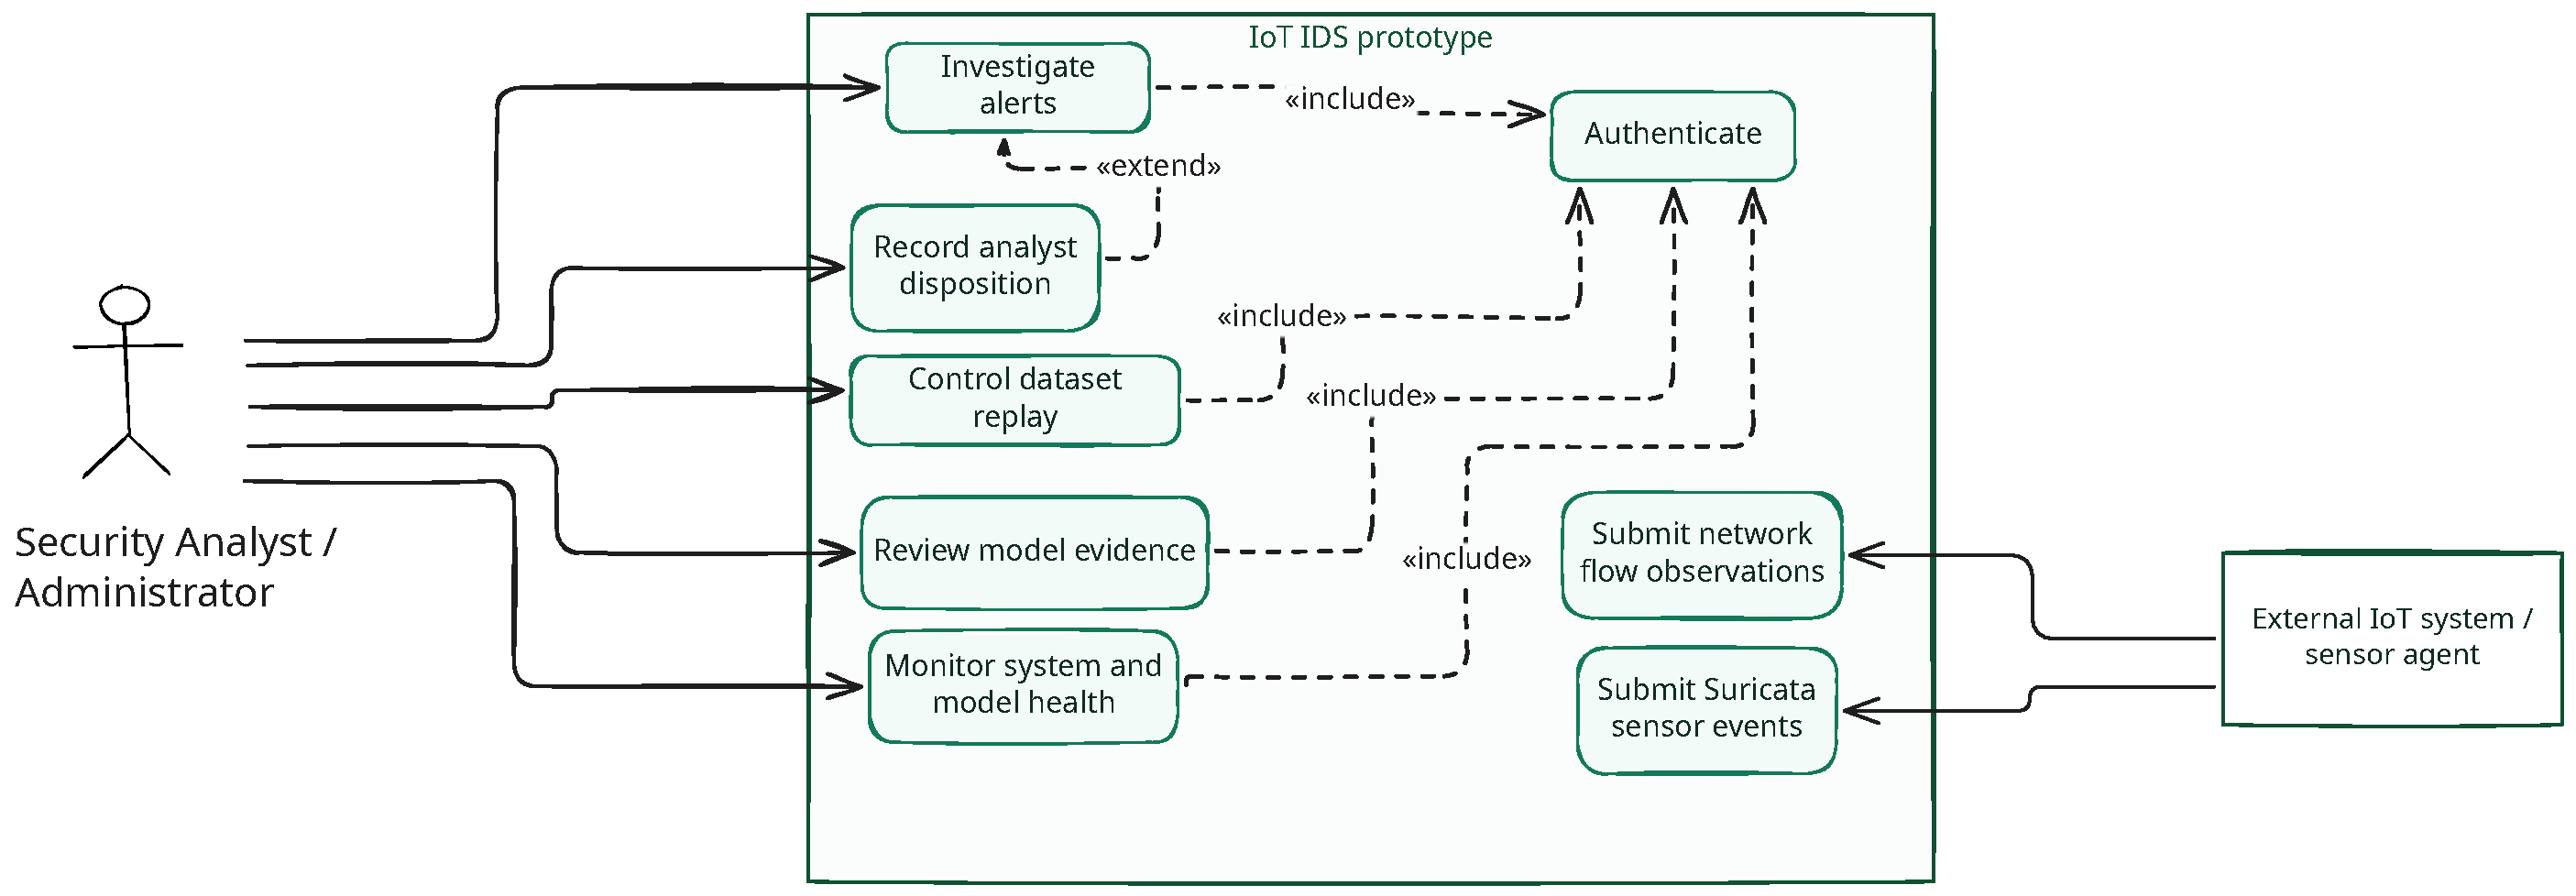
\includegraphics[
    width=\textwidth,
    height=.50\textheight,
    keepaspectratio
  ]{../diagrams/rendered/01-use-cases.pdf}
  \captionof{figure}{Cas d'utilisation du syst\`eme de d\'etection}
  \label{fig:use-cases}
\end{center}
\end{samepage}

\clearpage
\section{Description des cas d'utilisation}

Les tableaux suivants d\'ecrivent les parcours qui poss\`edent des validations,
des alternatives ou des effets persistants. Les chemins machine et op\'erateur
restent s\'epar\'es.

\subsection{UC-01 --- Authenticate}

\renewcommand{\arraystretch}{1.22}
\begin{longtable}{@{}>{\raggedright\arraybackslash}p{0.22\textwidth}>{\raggedright\arraybackslash}p{0.70\textwidth}@{}}
  \caption{Description du cas UC-01 --- Authenticate}\label{tab:uc-auth}\\
  \arrayrulecolor{SoftRule}\toprule
  \UCRow{Acteur}{Security Analyst / Administrator}
  \UCRow{Objectif}{Obtenir une session autoris\'ee sans exposer le secret.}
  \UCRow{Pr\'econditions}{L'authentification est configur\'ee et l'interface conna\^it son \'etat public.}
  \UCRow{Postconditions}{Un jeton à dur\'ee limit\'ee identifie l'op\'erateur; aucune donn\'ee m\'etier n'est modifi\'ee.}
  \UCRow{Sc\'enario nominal}{1. L'op\'erateur ouvre la connexion. 2. Il saisit ses identifiants. 3. L'API v\'erifie le secret. 4. L'interface affiche l'identit\'e et l'expiration retourn\'ees.}
  \UCRow{Alternatives}{Identifiants invalides: refus sans session. Tentatives trop nombreuses: refus temporaire avec d\'elai de reprise. Session expir\'ee: nouvelle authentification requise.}
  \bottomrule
\end{longtable}

\subsection{UC-02 --- Submit network flow observations}

\renewcommand{\arraystretch}{1.22}
\begin{longtable}{@{}>{\raggedright\arraybackslash}p{0.22\textwidth}>{\raggedright\arraybackslash}p{0.70\textwidth}@{}}
  \caption{Description du cas UC-02 --- Submit network flow observations}\label{tab:uc-ingestion}\\
  \arrayrulecolor{SoftRule}\toprule
  \UCRow{Acteur}{External IoT system / sensor agent utilisant le contrat d'observation autoris\'e.}
  \UCRow{Objectif}{Soumettre d'une à mille observations canoniques à la file durable.}
  \UCRow{Pr\'econditions}{Jeton autoris\'e; sch\'ema et version reconnus; identifiant d'\'ev\'enement fourni.}
  \UCRow{Postconditions}{Chaque nouvelle observation accept\'ee poss\`ede un travail en file et une transition initiale; un doublon identique reste idempotent.}
  \UCRow{Sc\'enario nominal}{1. Le producteur envoie JSON ou NDJSON. 2. L'API valide la requ\^ete enti\`ere. 3. Elle contr\^ole identit\'es et capacit\'e. 4. Elle ins\`ere les travaux dans une transaction. 5. Elle retourne le re\c{c}u du lot.}
  \UCRow{Alternatives}{Requ\^ete invalide: aucun travail stock\'e. M\^eme identifiant avec contenu diff\'erent: conflit. File satur\'ee: refus temporaire avec indication de reprise.}
  \bottomrule
\end{longtable}

\subsection{UC-03 --- Submit Suricata sensor events}

\renewcommand{\arraystretch}{1.22}
\begin{longtable}{@{}>{\raggedright\arraybackslash}p{0.22\textwidth}>{\raggedright\arraybackslash}p{0.70\textwidth}@{}}
  \caption{Description du cas UC-03 --- Submit Suricata sensor events}\label{tab:uc-suricata}\\
  \arrayrulecolor{SoftRule}\toprule
  \UCRow{Acteur}{External IoT system / sensor agent.}
  \UCRow{Objectif}{Transmettre une alerte de signature et l'\'etat observ\'e du capteur.}
  \UCRow{Pr\'econditions}{Jeton capteur valide; message EVE pris en charge; identifiant externe pr\'esent.}
  \UCRow{Postconditions}{L'alerte et l'\'etat du capteur sont persist\'es; un \'ev\'enement temps r\'eel est produit apr\`es validation.}
  \UCRow{Sc\'enario nominal}{1. L'agent lit un \'ev\'enement Suricata. 2. Il le normalise. 3. L'API authentifie la machine. 4. Elle d\'eduplique et persiste les preuves. 5. Elle retourne un re\c{c}u.}
  \UCRow{Alternatives}{Jeton absent ou invalide: refus. Message non conforme: erreur de validation. Identifiant d\'ej\`a accept\'e: traitement idempotent sans seconde alerte.}
  \bottomrule
\end{longtable}

\subsection{UC-04 --- Control dataset replay}

\renewcommand{\arraystretch}{1.22}
\begin{longtable}{@{}>{\raggedright\arraybackslash}p{0.22\textwidth}>{\raggedright\arraybackslash}p{0.70\textwidth}@{}}
  \caption{Description du cas UC-04 --- Control dataset replay}\label{tab:uc-replay}\\
  \arrayrulecolor{SoftRule}\toprule
  \UCRow{Acteur}{Security Analyst / Administrator.}
  \UCRow{Objectif}{Ex\'ecuter un rejeu born\'e et en contr\^oler la cadence.}
  \UCRow{Pr\'econditions}{Session valide; jeu pr\'epar\'e disponible; aucun autre rejeu actif.}
  \UCRow{Postconditions}{Les lignes trait\'ees restent persist\'ees; l'\'etat final indique ach\`evement ou arr\^et.}
  \UCRow{Sc\'enario nominal}{1. L'op\'erateur choisit sc\'enario, d\'ecalage, limite et vitesse. 2. L'API accepte la configuration. 3. Le serveur filtre et traite les lignes. 4. L'interface suit la progression.}
  \UCRow{Alternatives}{Configuration hors limites: refus. Rejeu actif: conflit. Pause: traitement suspendu. Reprise: cadence valid\'ee puis poursuite. Arr\^et: abandon du reste sans annuler les lignes d\'ej\`a trait\'ees.}
  \bottomrule
\end{longtable}

\subsection{UC-05 --- Investigate alerts and record disposition}

\renewcommand{\arraystretch}{1.22}
\begin{longtable}{@{}>{\raggedright\arraybackslash}p{0.22\textwidth}>{\raggedright\arraybackslash}p{0.70\textwidth}@{}}
  \caption{Description du cas UC-05 --- Investigate alerts and record disposition}\label{tab:uc-alert}\\
  \arrayrulecolor{SoftRule}\toprule
  \UCRow{Acteur}{Security Analyst / Administrator.}
  \UCRow{Objectif}{Examiner une alerte puis, si n\'ecessaire, enregistrer une qualification justifi\'ee.}
  \UCRow{Pr\'econditions}{Session valide; alerte persist\'ee.}
  \UCRow{Postconditions}{La consultation ne modifie pas l'alerte; une qualification confirm\'ee ajoute une entr\'ee immuable associ\'ee à l'identit\'e authentifi\'ee.}
  \UCRow{Sc\'enario nominal}{1. L'op\'erateur filtre la liste. 2. Il ouvre une alerte. 3. Il examine provenance, mod\`ele ou signature et explication disponible. 4. Il choisit un statut. 5. Il confirme la justification.}
  \UCRow{Alternatives}{Alerte absente: signalement sans modification. Explication indisponible: les autres preuves restent consultables. Justification obligatoire manquante: qualification refus\'ee.}
  \bottomrule
\end{longtable}

\subsection{UC-06 --- Monitor system and model health}

\renewcommand{\arraystretch}{1.22}
\begin{longtable}{@{}>{\raggedright\arraybackslash}p{0.22\textwidth}>{\raggedright\arraybackslash}p{0.70\textwidth}@{}}
  \caption{Description du cas UC-06 --- Monitor system and model health}\label{tab:uc-health}\\
  \arrayrulecolor{SoftRule}\toprule
  \UCRow{Acteur}{Security Analyst / Administrator.}
  \UCRow{Objectif}{Examiner l'\'etat des composants, de l'ingestion, du capteur et des cohortes de mod\`eles.}
  \UCRow{Pr\'econditions}{Application accessible; session valide pour les preuves m\'etier prot\'eg\'ees.}
  \UCRow{Postconditions}{Aucun \'etat m\'etier n'est modifi\'e; l'interface restitue l'instantan\'e et sa port\'ee.}
  \UCRow{Sc\'enario nominal}{1. L'op\'erateur ouvre la supervision. 2. L'interface charge sant\'e, file, capteur et cohortes. 3. Il choisit une cohorte et une fen\^etre. 4. Le syst\`eme retourne l'instantan\'e et l'historique disponibles.}
  \UCRow{Alternatives}{Composant indisponible: raison explicite. Instantan\'e absent ou observations insuffisantes: \'etat non concluant, sans pr\'etendre à une d\'erive mesur\'ee.}
  \bottomrule
\end{longtable}

\section{Conclusion}

Les besoins distinguent clairement les actions humaines, les entr\'ees machine
et les garanties transversales. Cette base permet de relier chaque parcours aux
composants, donn\'ees et interactions d\'ecrits dans le chapitre de conception.
